\chapter{Tensor Network Method}\label{chap:intro_ten}
\markboth{\MakeUppercase {Chapter \thechapter. \ Tensor Network Method}}{}

\section{Tensor Network group}
\markright{\MakeUppercase {\thechapter.\ Tensor Network group}}
In the tensor network methods,the partition function or 
the wave function is represented by large tensors ,and decomposed into
small tensors by singular value decomposition.We can get new tensor 
by constracting decomposed small tensors.Decomposing and constracting are
fundamental approah in the tensor network method.For example,I review Levin and Nave`s approah.

\begin{figure}[htb]
\centering
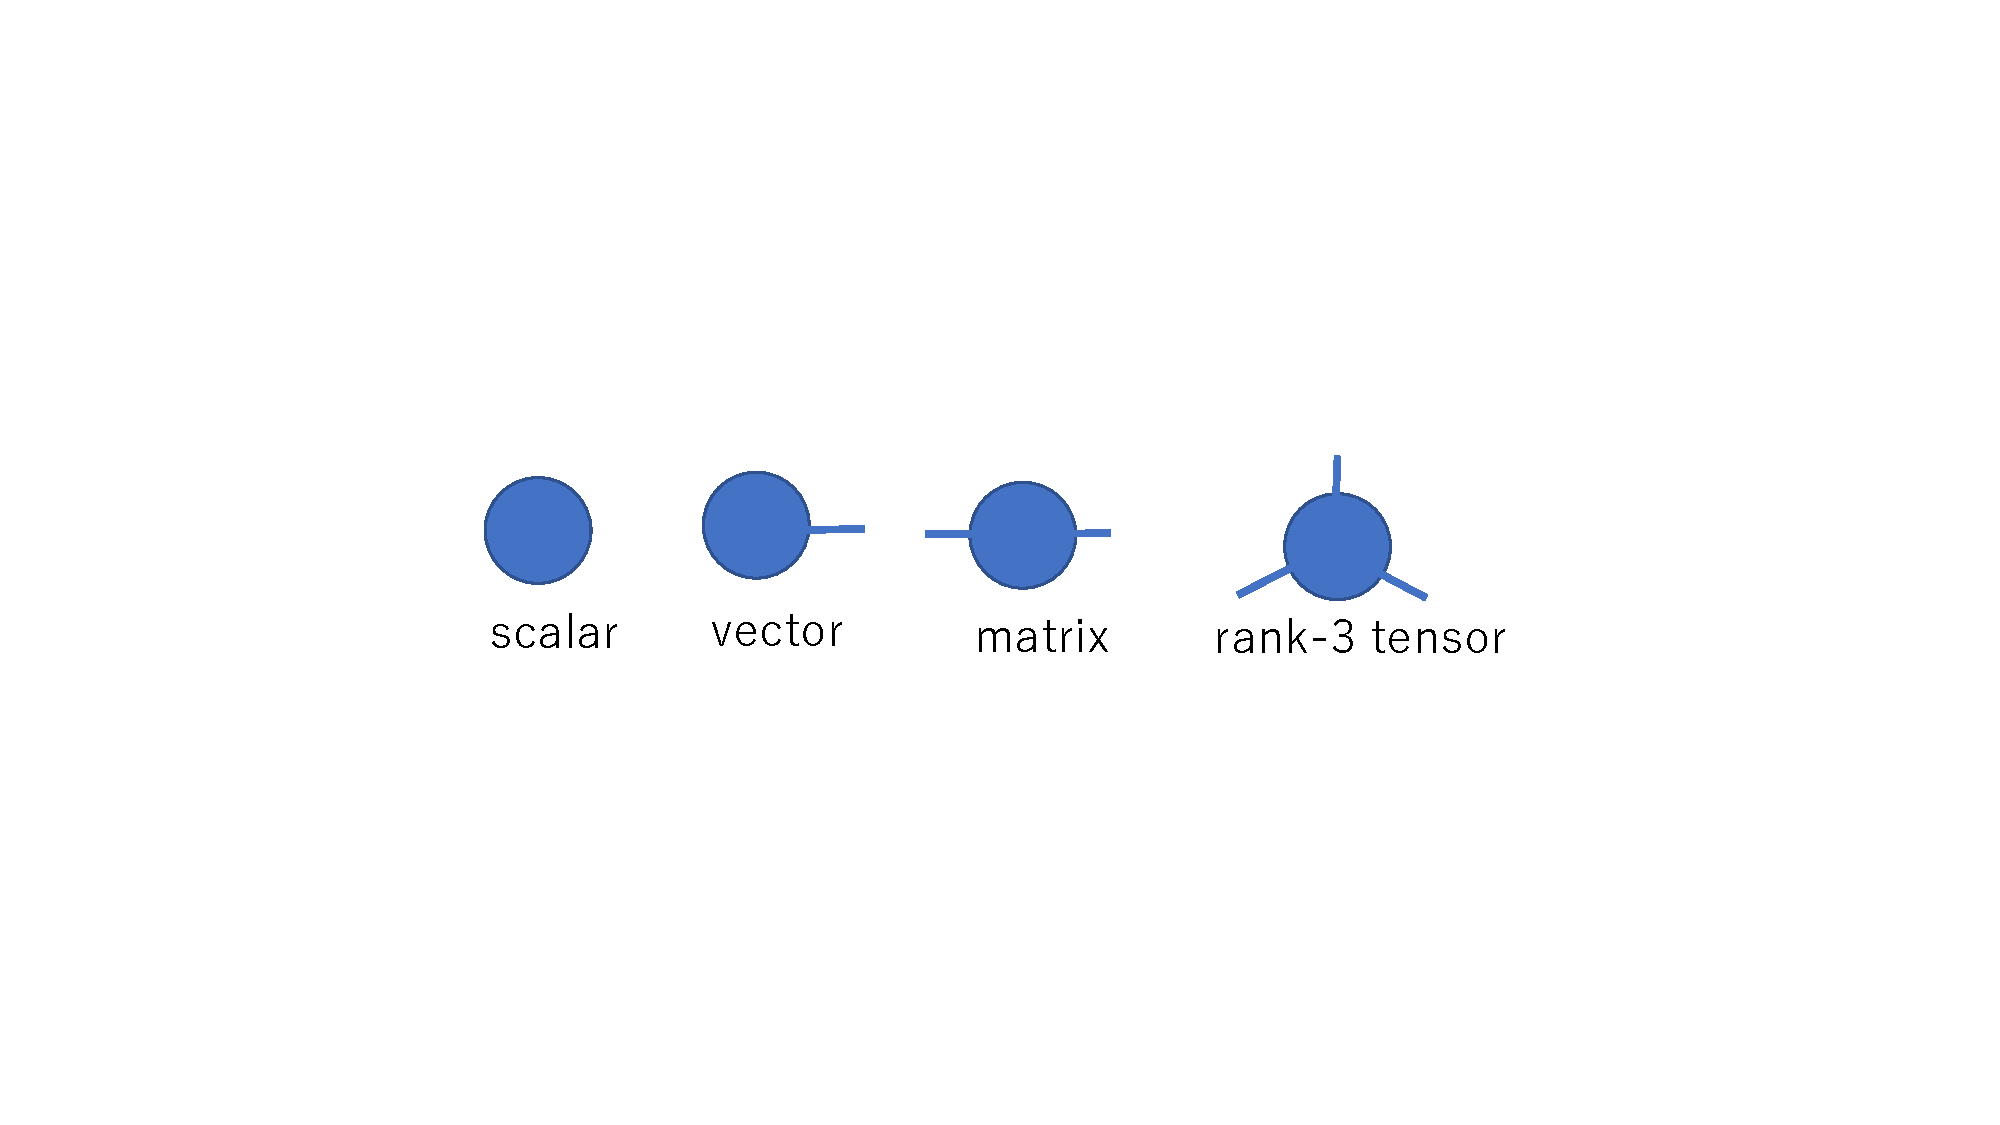
\includegraphics[clip,width=\hsize]{figure/tensor_index.pdf}
\caption{The diag}
\end{figure}

\section{Tensor renormalization group}
\markright{\MakeUppercase {\thechapter.\ Tensor renormalization group}}
Levin and Nave developed the tensor renormalization group(TRG)\cite{Levin-Nave2007}.
They applicate two-dimensional ising model.

\subsection{Singular value decomposition}
\markright{\MakeUppercase {\thechapter.\ Tensor renormalization group}}

